\documentclass[12pt,a4paper]{article}
\usepackage[latin1]{inputenc}
\usepackage{amsmath}
\usepackage{amsfonts}
\usepackage{amssymb}
\usepackage{graphicx}
\author{Luca Conterio - 920261\\  
	Ibrahim El Shemy - 920174}
\date{A.Y. 2018/2019 - Prof. Di Nitto Elisabetta}


\title{%
	\textbf{TrackMe} \\
	\large Requirements Analysis and Specification Document
}

\begin{document}
	
	\begin{figure}
		\centering
		
\includegraphics[width=1.0\linewidth]{images/polimi.jpg}
	\end{figure}
	
	\maketitle
	
	\newpage
	\tableofcontents
	\newpage
	
	\section{Introduction}
		\subsection{Purpose}
		This document represents the \texttt{Requirement Analysis and Specification Document} (RASD) for TrackMe software. Main goals of this project are to specify a system that will be able to store and analyze users' health data and whereabouts, to grant third parties to access these data or to subscribe to new data of a specific individual or to retrieve them, and to offer elderly people a rapid assistance based on their health parameters, if needed.
		At the same time, this document aims at describing the system through functional and nonfunctional requirements, to analyze customers' needs, to show the limits of the software, indicating the typical use cases that can occur.
	
	
	\subsection{Scope}
		\texttt{TrackMe} is a company that wants to develop a software-based service allowing third parties to monitor the location and health status of individuals.
		Hence, the system has to be composed by two specific services:
		\begin{itemize}
			\item \textbf{Data4Help}\\\\This service supports the registration of individuals who agree that TrackMe acquires their data (through electronic devices such as smartwatches). \\In addition, it supports the registration of third parties that can request:
			\begin{itemize}
				\item Access to the data of some specific individuals, who can accept/refuse it.
				\item Access to anonymized data of groups of individuals. These requests are approved by TrackMe if it is able to properly anonymize the requested data. The request is rejected if it is way too specific.
			\end{itemize}
			As soon as a request for some certain data is approved, TrackMe makes the previously saved data available to the third party. Also, it allows the third party to subscribe to new data and to receive them as soon as they are produced.
			\item \textbf{AutomatedSOS}\\\\This service is oriented to elderly people: monitoring their health status parameters, the system can send to the location of the customer an ambulance when some parameters are below certain thresholds, guaranteeing a reaction time of less than 5 seconds from the time the parameters get lower than the threshold.
		\end{itemize} 
	
		\subsubsection{Goals}
			\begin{itemize}
				\item {\textbf[}\textbf{G1}{\textbf]}: Allow visitors to easily register in the system.
				\item {\textbf[}\textbf{G2}{\textbf]}: Allow users to simply share personal information/health parameters.
				\item {\textbf[}\textbf{G3}{\textbf]}: Allow third parties to access information shared by users.
				\begin{itemize}
					\item {[G3.1]}: Allow third parties to access information of specific individuals (through an identifier).
					\item {[G3.2]}: Allow third parties to access anonymized information of groups of individuals.
					\item {[G3.3]}: Allow third parties to subscribe to new information of a specific individual and to receive it.
				\end{itemize}
				\item {\textbf[}\textbf{G4}{\textbf]}: Allow third parties to monitor specific users' parameters.
				\item {\textbf[}\textbf{G5}{\textbf]}: Guarantee the elderly users to receive an immediate assistance by an ambulance in case of high risk disease.
				\item {\textbf[}\textbf{G6}{\textbf]}: Guarantee the preservation of the privacy of the users.
			\end{itemize}
	
	
	\subsection{Definitions, Acronyms and Abbreviations}
		\subsubsection{Definitions}
		\subsubsection{Acronyms}
			\begin{itemize}
				\item RASD: Requirements Analysis and Specification Document.
				\item API: Application Programming Interface.
				\item GPS: Global Positioning System.
				\item SMS: Short Message Service. 
				\item ETA: Estimated Time Arrival.
				\item RAPS: Reliable Array of Partioned Service.
				\item SSN: Social Security Number.
			\end{itemize}
		\subsubsection{Abbreviations}
			\begin{itemize}
				\item {[}Gn{]}: n-goal.
				\item {[Rn]}: n-requirment.
				\item {App}: application.
			\end{itemize}
	
	\subsection{Document Structure}
		This paper refers to the structure suggested by IEEE for RASD documents, with very slight modifications:
		\begin{enumerate}
			\item \texttt{Introduction}: the first section is a general description of the system's scope and its goals. It also includes the revision history of the document and its references. Definitions and abbreviations used along the paper are provided too.
			\item \texttt{Overall Description}: this section includes shared phenomena, requirements and domain assumptions. It also clarifies users' needs.
			\item \texttt{Specific Requirements}: this section includes all the requirments, both functional and non functional.
			\item \texttt{Formal Analysis Using Alloy}: it includes the Alloy model of the described system.
			\item \texttt{Effort Spent}: this section includes information about the hours spent to draft this document. 
			\item \texttt{References}: this section includes references about papers/documents used to support this document.
		\end{enumerate}
	
	\newpage
	\section{Overall Description}
	
	\subsection{Product Perspective}
		\begin{figure}[h]
			%\centering
			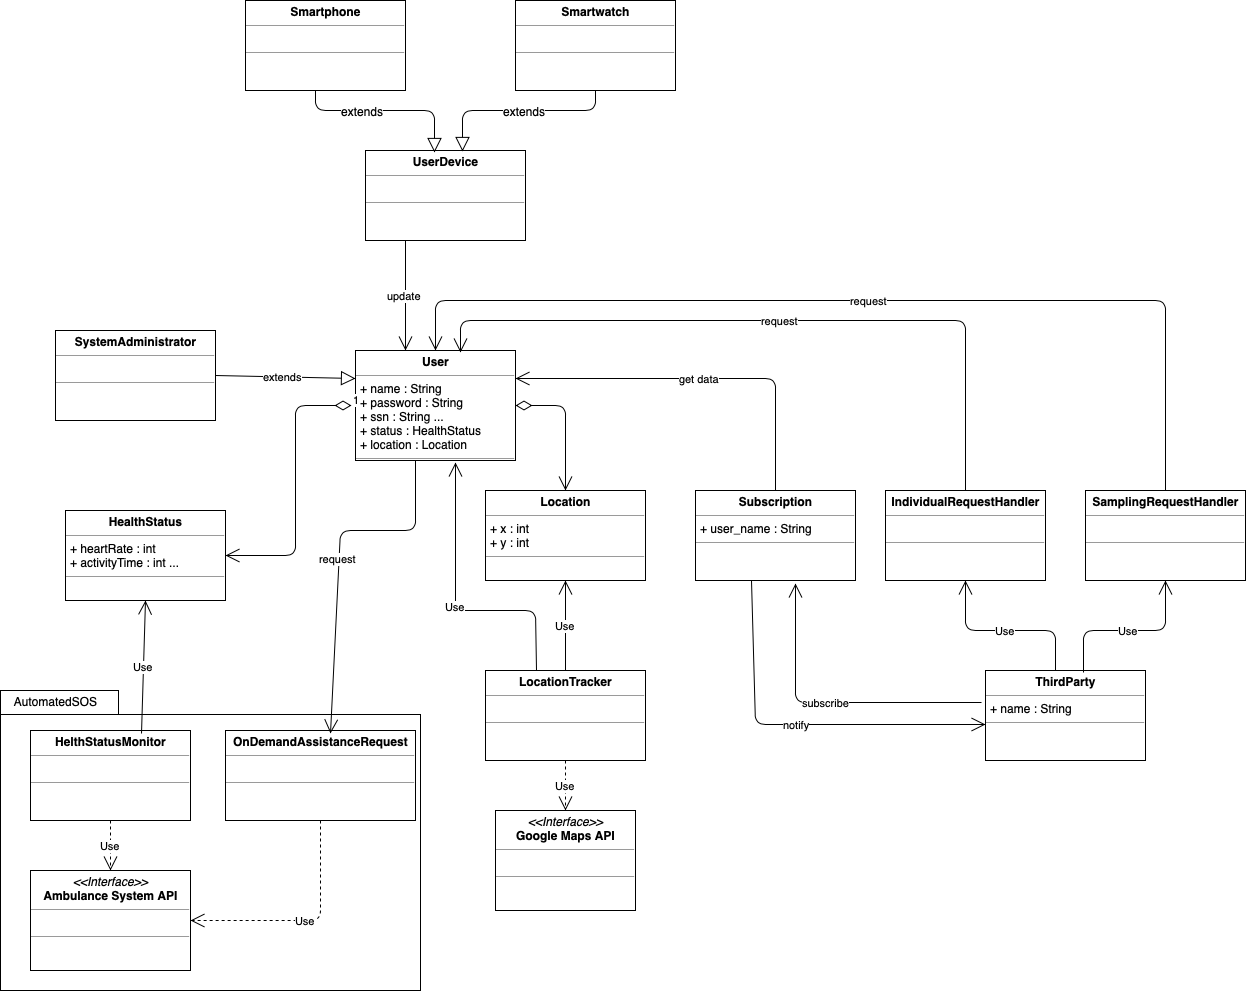
\includegraphics[width=1.25\linewidth]{Images/uml}
			\caption{UML Class Diagram}
			\label{fig:uml}
		\end{figure}
		\begin{figure}[H]
			%\centering
			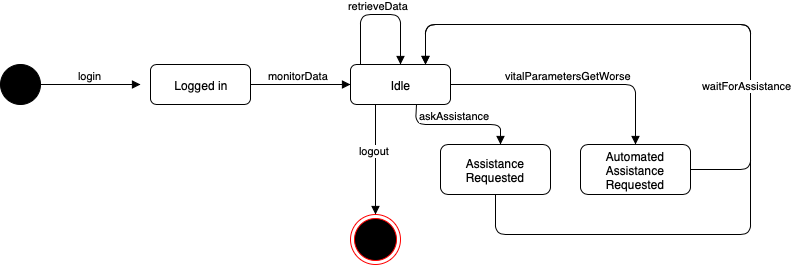
\includegraphics[width=1.0\linewidth]{Images/statechart_user}
			\caption{User Statechart Diagram}
			\label{fig:statechart_user}
		\end{figure}
		\begin{figure}[H]
			%\centering
			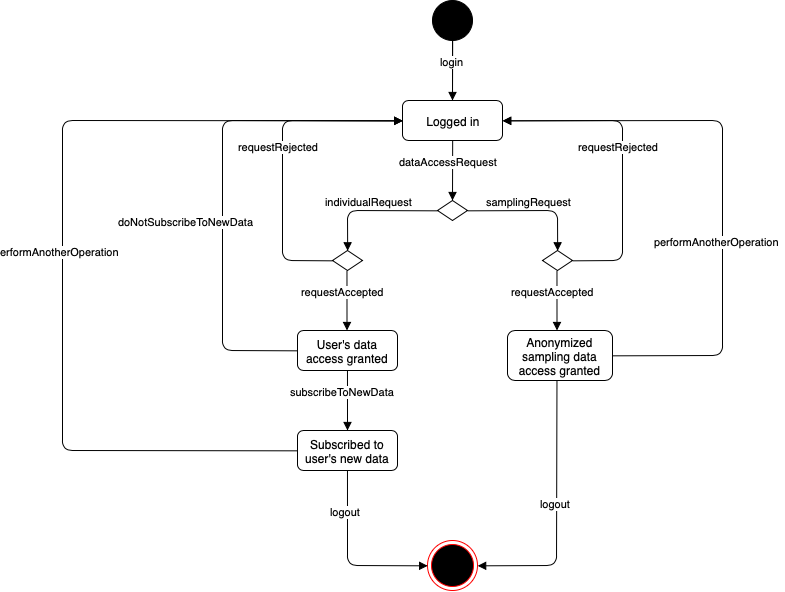
\includegraphics[width=1.0\linewidth]{Images/statechart_third_party}
			\caption{Third Party Statechart Diagram}
			\label{fig:statechart_third_party}
		\end{figure}
	
	\newpage
	\subsection{Product Functions}
	
	\subsection{User Characteristics}
		\begin{itemize}
			\item \texttt{Visitor}: a person visiting TrackMe without being registered. He can only proceed to registration in oder to actually use system services, otherwise he can't have access to any service or data.
			\item \texttt{System Administrator}: doesn't require to register himself. Makes sure there are no issues in the interaction between users and third parties, guaranteeing a certain level of security.
			\item \texttt{Registered user}: called simply \texttt{user} in this document. A person who registered himself to TrackMe, sharing his personal data. He can login to the system through provided credentials to exploit full services.
			\item \texttt{Third party user}: called simply \texttt{third party} in this document. A company or invidual using the platform for some statistical goal or to offer assistance to registered users.
			\item \texttt{Ambulance Dispatcher}: called simply \texttt{dispatcher} in this document. An external individual to the system, whose role is to dispatch an ambulance to assist specific users.
		\end{itemize}
	
	\subsection{Assumptions, Dependencies and Constraints}
		\subsubsection{Text Assumptions}
			\begin{itemize}
				\item In order to get registered, a Visitor must provide the following data: Name, Surname, Social Security Number, Date of Birth, Mobile Number, e-mail.
				\item In order to get registered, visitor must provide the following data: Name, Surname, Social Security Number, Date of Birth, Mobile Number, e-mail.
				\item Registration must be confirmed through a security code sent by SMS.
				\item Users are assumed to provide correct personal data (Name, Date of Birth, Social Security Number, etc.).
				\item Users are assumed to provide a valid Mobile Number and e-mail.
				\item Users' devices must support the Mobile Application.
				\item Users' devices must support the GPS technology.
				\item Users provide correct clinical data (such as blood group, allergies, etc.).
			\end{itemize}
		\subsubsection{Domain Assumptions}
			\begin{itemize} 
				\item {\textbf[}\textbf{D1}{\textbf]}: Social Security Number must be unique.
				\item {\textbf[}\textbf{D2}{\textbf]}: The verification message sent by SMS/e-mail will be certainly received by the User.
				\item {\textbf[}\textbf{D3}{\textbf]}: Users' devices are up and running in order to retrieve and process data. 
				\item {\textbf[}\textbf{D4}{\textbf]}: Data received (such as current location) by users' mobile devices are assumed to be correct.
				\item {\textbf[}\textbf{D5}{\textbf]}: Users' devices must support the Mobile Application.
				\item {\textbf[}\textbf{D6}{\textbf]}: Parameters provided by Users' are assumed to be correct.
				\item {\textbf[}\textbf{D7}{\textbf]}: The time spent by an ambulance to reach a defined location must be as low as possibile.
				\item {\textbf[}\textbf{D8}{\textbf]}: Users' devices are assumed to communicate through the Internet.
				\item {\textbf[}\textbf{D9}{\textbf]}: In case of emergency, all parameters relative to a specific individual are correctly reported to the ambulance dispatching system.
				\item {\textbf[}\textbf{D10}{\textbf]}: The Ambulance Dispatching System is always running and available.
				\item {\textbf[}\textbf{D11}{\textbf]}: The time spent by an ambulance to reach a defined location must be as low as possible.
				\item {\textbf[}\textbf{D12}{\textbf]}: The time spent by an ambulance to reach a defined location must be as low as possibile.
			\end{itemize}
		\subsubsection{Dependencies and Constraints}
			\begin{enumerate}
				\item Regulatory Policies:
				Guarantee confidentiality of information.
				\item Hardware Limitations: 
				\begin{itemize}
					\item \texttt{Mobile App}: iOS/Android, Internet Connection, GPS.
					\item \texttt{AppleWatch/WearOS}: smartwatches linked to mobile devices or equipped with GPS and equipped with hearbeat/pressure sensors.
					\item \texttt{Web App}: browser (e.g. Google Chrome / Safari) able to retrieve users' location.
				\end{itemize}
				\item Interfaces to other Applications: 
				\begin{itemize}
					\item API to ambulance dispatching system.
					\item API to external applications that monitor users health and activity parameters. (???)
					\item Google Maps API to have a visual representation of user location.
				\end{itemize}
			\end{enumerate}
	
	\newpage
	\section{Specific Requirements}
		\subsection{External Interface Requirments}
			\subsubsection{User Interfaces}
				The following mockups represt a basic idea of how the mobile application is supposed to look like.\\
				\begin{figure}[h]
					\centering
					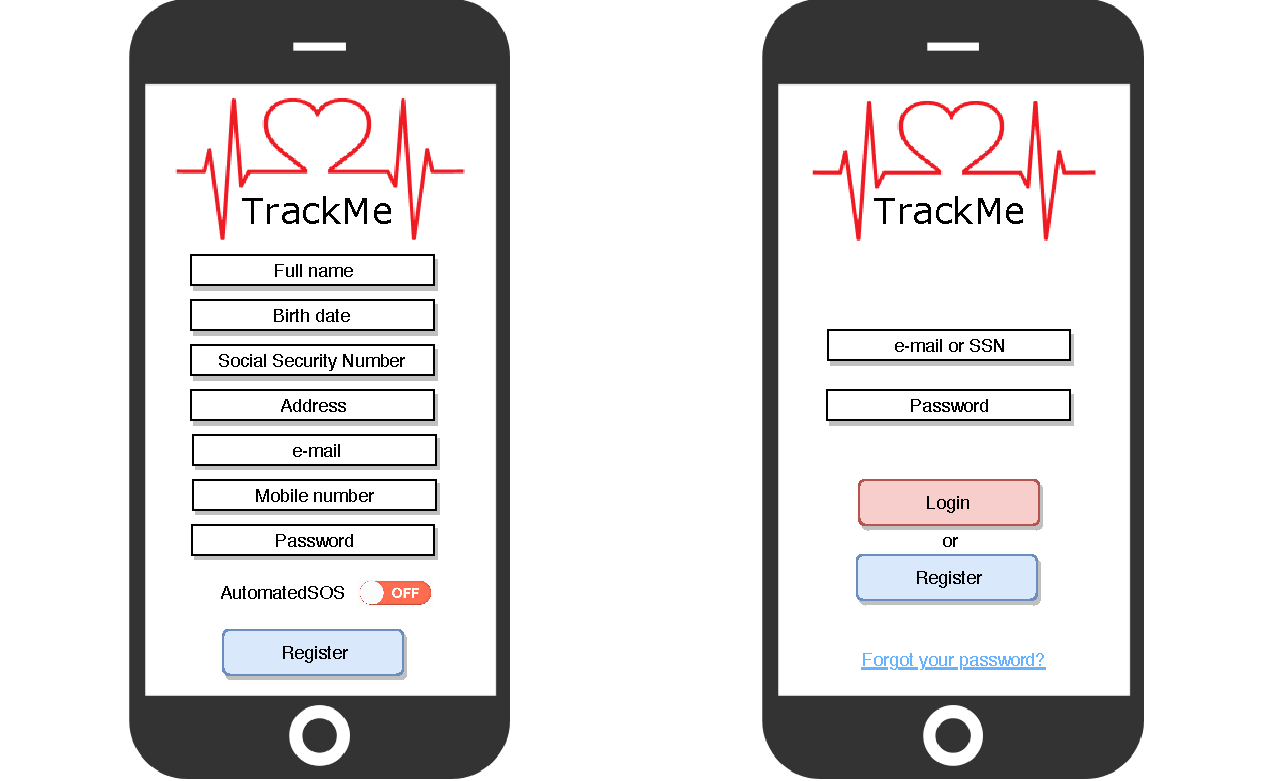
\includegraphics[width=1.0\linewidth]{Images/login-registration}
					\caption{Mobile App Registration form and login page}
					\label{fig:login-registration}
				\end{figure}
				\begin{figure}[H]
					\centering
					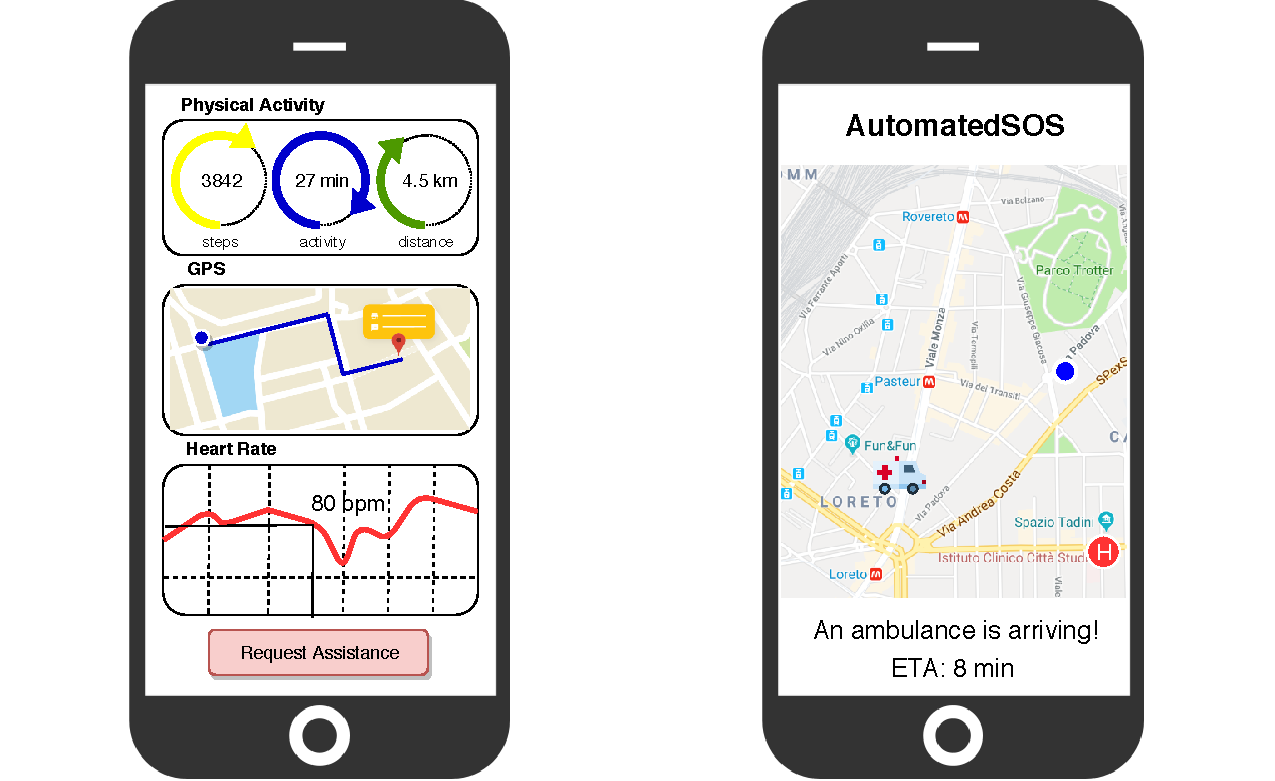
\includegraphics[width=1.0\linewidth]{Images/pages}
					\caption{Mobile app homepage with activity data, AutomatedSOS interface during an ambulance request and personal data pages.}
					\label{fig:pages}
				\end{figure}
			
			\newpage
			\subsubsection{Hardware Interfaces}
			\subsubsection{Software Interfacse}
			\subsubsection{Communication Interfaces}
			
		\subsection{Scenarios}
			
	\newpage
	
	\subsection{Functional Requirments}
		
		\subsubsection*{{[}{G1}{]}: Allow visitors to easily register in the system}
			\begin{itemize}
				\begin{itemize}
					\item {[D1]}: The SSN must be unique.
					\item {[D2]}: The verification message sent by SMS/e-mail will be certainly received by the User/Third Party.
					\\\\
					\item {[R1]}: The system must allow the Visitor/Third Party to provide credentials and personal data.
					\item {[R2]}: The system must verify the correspondance between the SSN provided by the Visitor/Third Party and their personal information.
					\item {[R3]}: The system must verify the correctness of the data provided by the Visitor/Third Parties with an e-mail/SMS verification.
					\item {[R4]}: The system must verify that there are no other registered Users/Third Parties with the same SSN/e-mail.
					\item {[R5]}: In order to register successfully a Third Party, the system must oblige it to accept data privacy conditions.
				\end{itemize} 
			\end{itemize}
		\subsubsection*{{[}{G2}{]}: Allow Users to share personal information/health parameters}
			\begin{itemize}
				\begin{itemize}
					\item {[D3]}: Users' devices are up and running in order to retrieve and process data.
					\item {[D4]}: Users' devices must support the GPS technology.
					\item {[D5]}: Users' devices must support the Mobile Application
					\item {[D6]}: Data periodically received by Users' devices are assumed to have a good accuracy. 
					\item {[D7]}: Parameters provided by Users' are assumed to be correct. 
					\item {[D8]}: Users' devices are assumed to communicate throught the Internet.
					\\\\
					\item {[R6]}: Users locations are retrieved by GPS.
					\item {[R7]}: The system must allow the Users to update their personal data.
					\item {[R8]}: The system must allow the Users to upload their medical records (such as blood group).
				\end{itemize} 
			\end{itemize}
		\subsubsection*{{[}{G3}{]}: Allow Third Parties to access information shared by the Users}
			\begin{itemize}
				\item {[G3.1]}: Allow Third Parties to access information of specific individuals.
				\begin{itemize}
					\item {[R9]}: The system must allow Third Parties to search Users through their SSN's.
					\item {[R10]}: The system must allow Third Parties to send requests in order to access specific data.
					\item {[R11]}: The system must allow Users either to accept or refuse Third Parties' requests.
				\end{itemize} 
				
				\item {[G3.2]}: Allow Third Parties to access anonymized information and parameters of groups of individuals.
				\begin{itemize}
					\item {[R12]}:The system must allow Third Parties to perform samplings according to some parameters (such as Geographical ones).
					\item {[R13]}: The system must anonymize sampling result data.
					\item {[R14]}: The system must accept sampling if and only if results are related to more than 1000 Users.
				\end{itemize} 
				
				\item {[G3.3]}: Allow Third Parties to subscribe to new information of a specific individual and to receive it.
				\begin{itemize}
					\item {[R15]}: If a User accepts a requests, the system must allow Third Parties to store and access the previously saved data.
					\item {[R16]}: The system must show Third Parties new data whenever they are available.
				\end{itemize}
			\end{itemize}
		\subsubsection*{{[}{G4}{]}: Guarantee the elderly users to receive an immediate assistance by an ambulance in case of high risk disease}
			\begin{itemize}
				\begin{itemize}
					\item {[D6]}: Parameters periodically received by Users' devices are assumed to have a good accuracy. 
					\item {[D9]}: In case of emergency, all parameters relative to a specific individual are correctly reported to the ambulance dispatching system.
					\item {[D10]}: The ambulance dispatching system is always running and reliable.
					\item {[D12]}: The time spent by an ambulance to reach a defined location must be as low as possibile. 
					\\\\
					\item {[R16]}: The AutomatedSOS service is automatically activated during the registration process if the Visitor is over 60.
					\item {[R17]}: The Health Status Monitoring System must notify the Ambulance Dispatching System. 
					\item {[R18]}: When the Ambulance Dispatching System is notified, the Health Status Monitoring System sends all the User's clinical parameters.
					\item {[R19]}: The system should let the User have the possibily to request directly help from an ambulance if he feels it is necessary.
				\end{itemize}
			\end{itemize}
		\subsubsection*{{[}{G5}{]}: Guarantee the preservation of the privacy of the Users.}
			\begin{itemize}
				\begin{itemize}
					\item {[D2]}: Parameters periodically received by Users' devices are assumed to have a good accuracy. 
					\item {[D5]}: Data provided by Users' are assumed to be correct. 
					\\\\
					\item {[R5]}: In order to register successfully a Third Party, the system must oblige it to accept data privacy conditions.
					\item {[R8]}: A Third Party can access data and parameters of a specific User if and only if he/she accepts the request.
					\item {[R3]}: The system must accept sampling if and only if results are related to more than 1000 Users.
					\item {[R9]}: The system must implement some form of accurate access control on databases.
				\end{itemize}
			\end{itemize}
		
		\newpage
		\subsubsection{Visitor Use Case Diagram}
			\begin{figure}[h]
				\centering
				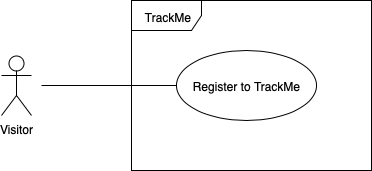
\includegraphics[width=0.7\linewidth]{Images/use_case_visitor}
				\label{fig:use_case_visitor}
			\end{figure}
		
		\subsubsection{User Use Case Diagram}
			\begin{figure}[h]
				\centering
				%\includegraphics[width=0.7\linewidth]{Images/use_case_user}
				\label{fig:use_case_user}
			\end{figure}
		
		\subsubsection{Third Party Use Case Diagram}
			\begin{figure}[h]
				\centering
			    %\includegraphics[width=0.7\linewidth]{Images/use_case_third_party}
				\label{fig:use_case_third_party}
			\end{figure}
		
		\subsubsection{System Manager Use Case Diagram ???}
		???????
	
	\subsection{Performance Requirments}
	The system must be able to handle a huge quantity of requests simultaneously throughout the day, responding to users' necessities in the shortest time possible. In order to improve the perfomance of the system, since data are received in a discrete way (e.g. monitored every 5 seconds), TrackMe relies on a UDP non-persistent connection.\\
	For what concerns the AutomatedSOS service, it is required that each ambulance request is generated and sent to the Ambulance Dispatching System within 5 seconds from the moment in which the vital parameters of an elder user get below the fixed threshold.
	
	\subsection{Desgin Constraints}
		\subsubsection{Standards Compliance}
		\subsubsection{Hardware Limitations}
		\subsubsection{Other Constraints}
	
	\subsection{Software System Attributes}
		\subsubsection{Reliability}
		The system must guarantee a 24/7 service. This requirment should not have any sort of deviation (especially concerning AutomatedSOS).
		\subsubsection{Availability}
		The system must fullfil all the requests whenever needed (e.g. get/update personal information, request for medical assistance). Only a small percentage of the total requests is admissible (less than 0.01\% of the total amount of requests). The system relies on a RAPS architecture, to better guarantee availability. The whole system is partitioned in nodes, each one managing a single service, in which data is made redudant in different servers. In this way, the malfuction of a service will not cause a service breakdown, but only a decrease of performance.
		\subsubsection{Security}
		Despite the fact that personal information is stored, the system guarantees not to spread them outside, and third parties are obliged to be confirmed with a privacy policy.
		\subsubsection{Maintainability}
		Enforced by the usage of specific design patterns (e.g. third party subscription is notified through an Observer Pattern whenever new data is generated by the users) and the provided documentation.
		\subsubsection{Scalability}
		Relying on a RAPS architecture, it is easier to enlarge the structure of the system, since it is possible to invest only on those services that need to handle the higher amount of requests or the ones where the number of users is relevant.
	
	
	\newpage
	\section{Formal Analysis Using Alloy}
	
	\newpage
	%\section{Appendix}
	%\subsection{Tools used}
	
	\section{Effort Spent}
	\begin{itemize}
		\item Luca Conterio
		\begin{center}
			\begin{tabular}{| c | c | c |}
				\hline
				Day & Subject & Hours \\ \hline
				15/10/2018 & Purpose, Scope and goals & 1 \\
				18/10/2018 & Overall Description & 1.5 \\
				19/10/2018  & User Interface sketch and Domain assumptioms & 2 \\
				22/10/2018  & UML and Non-Functional Requirements & 3.5 \\
				25/10/2018 & Functional Requirements & 3 \\
				26/10/2018 & Statechart Diagrams & 2 \\
				\hline
				Total & & 13\\
				\hline
			\end{tabular}
		\end{center}
		
		\item Ibrahim El Shemy
		\begin{center}
			\begin{tabular}{| c | c | c |}
				\hline
				Day & Subject & Hours \\ \hline
				15/10/2018 & Purpose, Scope and goals & 1 \\
				18/10/2018 & Overall Description & 1 \\
				19/10/2018  & Domain Assumptions & 2 \\
				22/10/2018  & Assumptions and Non-Functional Requirements & 3.5 \\
				25/10/2018 & Functional Requirements & 3 \\
				26/10/2018 & Functional Requirements & 1 \\
				\hline
				Total & & 11.5\\
				\hline
			\end{tabular}
		\end{center}
	\end{itemize}
	\section{Reference Documents}
	\begin{itemize}
		\item Specification Document "Mandatory Project Assignment A.Y. 2018/2019"
		\item 830-1993 - IEEE Recommended Practice for Software Requirements
		\item "Appunti di Sistemi Informativi per il Settore dell'Informazione" A.Y. 2017/2018
		Specifications
	\end{itemize}
\end{document}
